\documentclass[man]{apa6}
\usepackage{lmodern}
\usepackage{amssymb,amsmath}
\usepackage{ifxetex,ifluatex}
\usepackage{fixltx2e} % provides \textsubscript
\ifnum 0\ifxetex 1\fi\ifluatex 1\fi=0 % if pdftex
  \usepackage[T1]{fontenc}
  \usepackage[utf8]{inputenc}
\else % if luatex or xelatex
  \ifxetex
    \usepackage{mathspec}
  \else
    \usepackage{fontspec}
  \fi
  \defaultfontfeatures{Ligatures=TeX,Scale=MatchLowercase}
\fi
% use upquote if available, for straight quotes in verbatim environments
\IfFileExists{upquote.sty}{\usepackage{upquote}}{}
% use microtype if available
\IfFileExists{microtype.sty}{%
\usepackage{microtype}
\UseMicrotypeSet[protrusion]{basicmath} % disable protrusion for tt fonts
}{}
\usepackage{hyperref}
\hypersetup{unicode=true,
            pdftitle={Lab 8 APA Manuscript Using Papaja in R},
            pdfauthor={Lisa Strycker~\& Noah Strycker},
            pdfkeywords={tonic immobility},
            pdfborder={0 0 0},
            breaklinks=true}
\urlstyle{same}  % don't use monospace font for urls
\usepackage{graphicx,grffile}
\makeatletter
\def\maxwidth{\ifdim\Gin@nat@width>\linewidth\linewidth\else\Gin@nat@width\fi}
\def\maxheight{\ifdim\Gin@nat@height>\textheight\textheight\else\Gin@nat@height\fi}
\makeatother
% Scale images if necessary, so that they will not overflow the page
% margins by default, and it is still possible to overwrite the defaults
% using explicit options in \includegraphics[width, height, ...]{}
\setkeys{Gin}{width=\maxwidth,height=\maxheight,keepaspectratio}
\IfFileExists{parskip.sty}{%
\usepackage{parskip}
}{% else
\setlength{\parindent}{0pt}
\setlength{\parskip}{6pt plus 2pt minus 1pt}
}
\setlength{\emergencystretch}{3em}  % prevent overfull lines
\providecommand{\tightlist}{%
  \setlength{\itemsep}{0pt}\setlength{\parskip}{0pt}}
\setcounter{secnumdepth}{0}
% Redefines (sub)paragraphs to behave more like sections
\ifx\paragraph\undefined\else
\let\oldparagraph\paragraph
\renewcommand{\paragraph}[1]{\oldparagraph{#1}\mbox{}}
\fi
\ifx\subparagraph\undefined\else
\let\oldsubparagraph\subparagraph
\renewcommand{\subparagraph}[1]{\oldsubparagraph{#1}\mbox{}}
\fi

%%% Use protect on footnotes to avoid problems with footnotes in titles
\let\rmarkdownfootnote\footnote%
\def\footnote{\protect\rmarkdownfootnote}


  \title{Lab 8 APA Manuscript Using Papaja in R}
    \author{Lisa Strycker\textsuperscript{1,2}~\& Noah Strycker\textsuperscript{3}}
    \date{}
  
\shorttitle{Lab 8 Assignment}
\affiliation{
\vspace{0.5cm}
\textsuperscript{1} Oregon Research Institute\\\textsuperscript{2} University of Oregon\\\textsuperscript{3} Stony Brook University}
\keywords{tonic immobility}
\usepackage{csquotes}
\usepackage{upgreek}
\captionsetup{font=singlespacing,justification=justified}

\usepackage{longtable}
\usepackage{lscape}
\usepackage{multirow}
\usepackage{tabularx}
\usepackage[flushleft]{threeparttable}
\usepackage{threeparttablex}

\newenvironment{lltable}{\begin{landscape}\begin{center}\begin{ThreePartTable}}{\end{ThreePartTable}\end{center}\end{landscape}}

\makeatletter
\newcommand\LastLTentrywidth{1em}
\newlength\longtablewidth
\setlength{\longtablewidth}{1in}
\newcommand{\getlongtablewidth}{\begingroup \ifcsname LT@\roman{LT@tables}\endcsname \global\longtablewidth=0pt \renewcommand{\LT@entry}[2]{\global\advance\longtablewidth by ##2\relax\gdef\LastLTentrywidth{##2}}\@nameuse{LT@\roman{LT@tables}} \fi \endgroup}


\DeclareDelayedFloatFlavor{ThreePartTable}{table}
\DeclareDelayedFloatFlavor{lltable}{table}
\DeclareDelayedFloatFlavor*{longtable}{table}
\makeatletter
\renewcommand{\efloat@iwrite}[1]{\immediate\expandafter\protected@write\csname efloat@post#1\endcsname{}}
\makeatother

\authornote{

Correspondence concerning this article should be addressed to Lisa Strycker, Eugene, OR. E-mail: \href{mailto:lisas@ori.org}{\nolinkurl{lisas@ori.org}}}

\abstract{
Animal species have different behaviors for avoiding predators. Tonic immobility of a form of passive anti-predator behavior.

In tonic immobility, organisms do not respond to external stimulation.

Tonic immobility has been shown in isopods, including ``sow bugs,'' but is largely unstudied. This study answered four research questions: (a) Do species differ in responsiveness to tonic immobility-inducing stimuli? (b) Does the responsiveness depend upon sex, size, or stimulus? (c) Is the duration of tonic immobility influenced by sex, size, or type of stimulus, and does it differ between species? (d) Is the duration of tonic immobility related to the time needed to elicit a response?

Here we show that responses to external stimuli differ within and between three species of isopods. Three distinct patterns were found.

Relatively stronger responses to different stimuli (e.g., drop, touch) may be because some species tend to have visual predators that are larger or smaller than they are.


}

\begin{document}
\maketitle

\hypertarget{methods}{%
\section{Methods}\label{methods}}

Methods were similar to Quadros, Bugs, and Araujo (2012) and others (see Hoagland, 1927).

\hypertarget{participants}{%
\subsection{Participants}\label{participants}}

Participants were sow bugs and students in public school.

\hypertarget{material}{%
\subsection{Material}\label{material}}

Materials included forceps and teachers.

\hypertarget{procedure}{%
\subsection{Procedure}\label{procedure}}

All procedures were approved by the Institutional Review Board. Sow bugs were debriefed after each trial. Children were informed that they could withdraw from the study at any time.

\hypertarget{data-analysis}{%
\subsection{Data analysis}\label{data-analysis}}

Data were analyzed.

\hypertarget{results}{%
\section{Results}\label{results}}

Results showed differences by gender and socioeconomic status in math and reading scores (see table). Results also indicated a positive relationship between years of teacher experience and total math scale score. The pattern was the same regardless of socioeconomic status, but students who paid for meals had higher math scale scores overall (see plot).

\hypertarget{discussion}{%
\section{Discussion}\label{discussion}}

More studies are needed to investigative whether anti-predator strategies like tonic immobility improve survivorship. Future research should elucidate which responses work for different predators.
\newpage

\hypertarget{references}{%
\section{References}\label{references}}

\begingroup
\setlength{\parindent}{-0.5in}
\setlength{\leftskip}{0.5in}

\hypertarget{refs}{}
\leavevmode\hypertarget{ref-hoagland1927}{}%
Hoagland, H. (1927). Quantitative aspects of tonic immobility in vertebrates. \emph{Proceedings of the National Academy of Sciences of the United States of America}, \emph{13}(12), 838.

\leavevmode\hypertarget{ref-quadros2012}{}%
Quadros, A. F., Bugs, P. S., \& Araujo, P. B. (2012). Tonic immobility in terrestrial isopods: Intraspecific and interspecific variability. \emph{ZooKeys}, (176), 155.

\endgroup

\newpage

\begin{table}[H]
\centering
\begin{tabular}{l|l|r|r|r|r}
\hline
sex & frl & math\_mean & math\_sd & rdg\_mean & rdg\_sd\\
\hline
boy & no & 492.85 & 46.34 & 441.46 & 32.32\\
\hline
boy & yes & 469.87 & 46.09 & 425.38 & 26.63\\
\hline
girl & no & 501.21 & 45.96 & 448.54 & 34.52\\
\hline
girl & yes & 477.51 & 46.30 & 430.80 & 27.42\\
\hline
\end{tabular}
\end{table}

\newpage

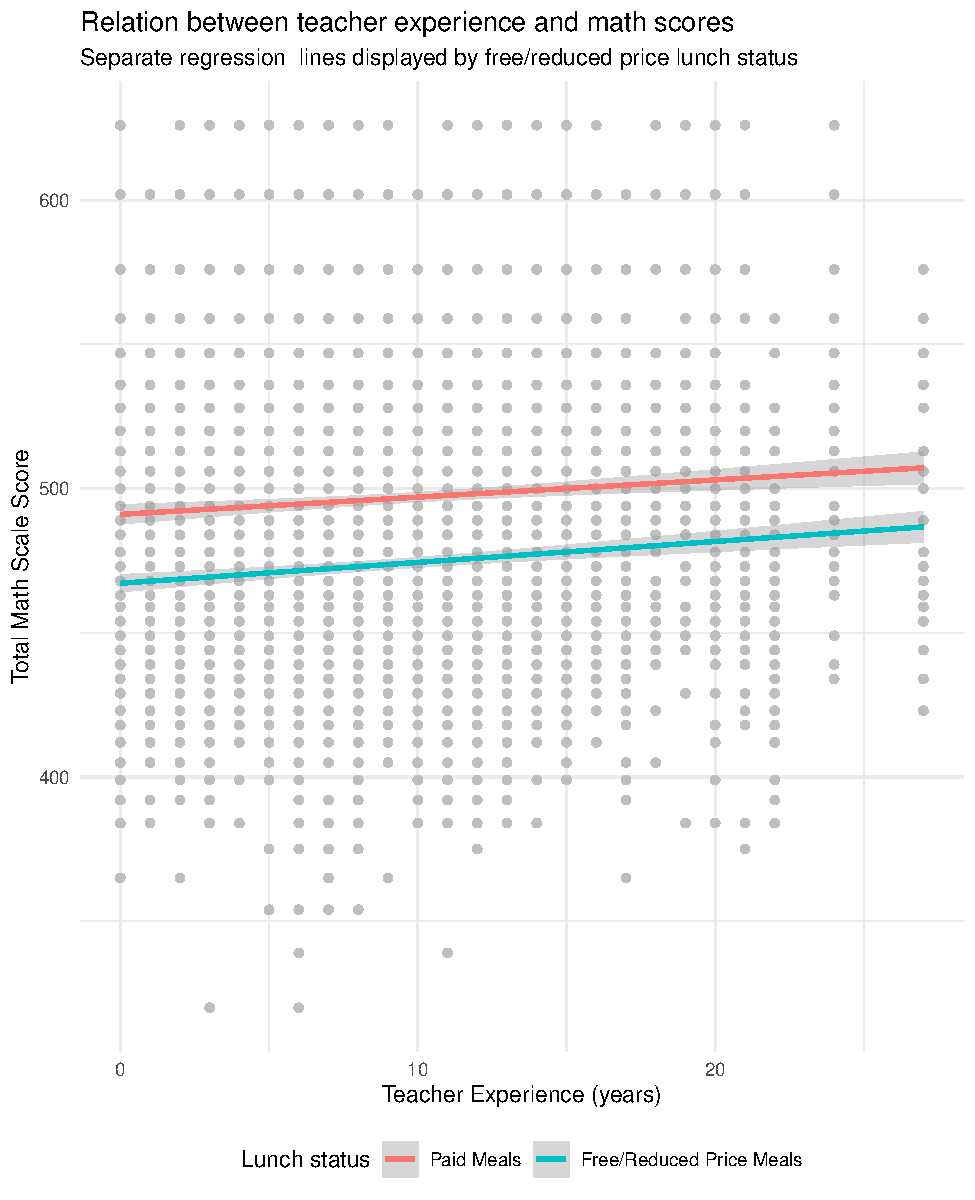
\includegraphics{lab_8a_files/figure-latex/create_graph-1.pdf}


\end{document}
